\documentclass[12pt,a4paper]{article}
\usepackage[brazil]{babel}
\usepackage[utf8]{inputenc}
\usepackage[T1]{fontenc}
\usepackage{lmodern}
\usepackage[top=2.5cm,bottom=2.5cm,left=3cm,right=2.5cm]{geometry}
\usepackage{graphicx}
\usepackage{booktabs}
\usepackage{amsmath}
\usepackage{hyperref}
\usepackage{float}
\usepackage{listings}
\usepackage{xcolor}
\usepackage{caption}
\usepackage{subcaption}
\usepackage{setspace}
\usepackage{indentfirst}
\usepackage{enumerate}

\onehalfspacing

\hypersetup{
  colorlinks=true,
  linkcolor=black,
  urlcolor=blue,
  citecolor=black
}

\lstset{
  language=Python,
  basicstyle=\small\ttfamily,
  keywordstyle=\color{blue}\bfseries,
  commentstyle=\color{gray},
  stringstyle=\color{orange},
  breaklines=true,
  frame=single,
  numbers=left,
  numberstyle=\tiny\color{gray},
  xleftmargin=1.5em,
  framexleftmargin=1.5em
}

\title{%
  \textbf{PGC308A -- Estimativa de Conformidade a SLAs}\\[0.3em]
  \large Relatório Final -- 2026/1
}
\author{
  Victor Guimarães Silva \and Raquel de Fátima Alves\\[0.3em]
  \small PPGCO/FACOM -- Universidade Federal de Uberlândia
}
\date{Junho de 2026}

\begin{document}
\maketitle
\thispagestyle{empty}

\begin{abstract}
Este relatório descreve a implementação e análise de modelos de aprendizado de máquina
supervisionado para estimar a conformidade a SLAs em um serviço de vídeo sob demanda (VoD).
O problema consiste em prever, a partir de métricas do servidor Linux, se o serviço atende
ao SLA definido como taxa mínima de frames no cliente ($\geq 18$ fps).
Foram implementadas três tasks: exploração dos dados (Task~I), regressão linear para
estimativa contínua dos fps (Task~II) e regressão logística para classificação binária
de conformidade (Task~III). Como atividade bônus, aplicou-se regressão linear à predição
de qualidade de sinal 5G em traces coletados em campo em São Paulo.
O código-fonte completo está disponível em:
\url{https://github.com/victorguimaraessilva/Trabalho-IA-MSc}.
\end{abstract}

\tableofcontents
\newpage

%% ============================================================
\section{Introdução}
%% ============================================================

Provedores de serviços de vídeo sob demanda (VoD) precisam garantir que os usuários
recebam qualidade satisfatória de reprodução. O \textit{Service Level Agreement} (SLA)
formaliza esse compromisso: neste trabalho, o SLA é definido como a taxa de frames
percebida pelo cliente (\texttt{DispFrames}) igual ou superior a 18 fps.
Medir diretamente a qualidade no terminal do usuário em tempo real é, em geral,
inviável em escala. A alternativa estudada neste trabalho é usar \textbf{aprendizado
de máquina supervisionado} para inferir a qualidade do cliente a partir de métricas
coletadas no próprio servidor -- uma prática conhecida como \textit{service assurance}.

O conjunto de dados contém 3.600 observações, uma por segundo, durante uma hora de operação.
As variáveis de entrada (X) descrevem o estado do servidor Linux (CPU, memória, processos,
rede, etc.) e a variável alvo (Y) é a taxa de frames observada no cliente (\texttt{DispFrames}).

Três tasks foram propostas: (I) exploração e análise dos dados; (II) regressão linear para
prever os fps com métrica NMAE; e (III) regressão logística para classificar o serviço como
\textit{conforme} ou \textit{em violação} do SLA com métrica ERR. Adicionalmente, foi
implementada a Atividade~A do 5G Datasets Challenge como bônus.

O repositório com todos os notebooks e código-fonte está disponível publicamente em:\\
\url{https://github.com/victorguimaraessilva/Trabalho-IA-MSc}

%% ============================================================
\section{Dados e Metodologia}
%% ============================================================

\subsection{Descrição dos Dados}

O dataset é composto por dois arquivos:
\begin{itemize}
  \item \textbf{X.csv}: 9 métricas do servidor Linux, amostradas a cada segundo;
  \item \textbf{Y.csv}: taxa de frames no cliente (\texttt{DispFrames}, em fps), no mesmo instante.
\end{itemize}

A Tabela~\ref{tab:variaveis} descreve cada variável de entrada.

\begin{table}[H]
\centering
\caption{Variáveis de entrada (servidor) e variável alvo (cliente).}
\label{tab:variaveis}
\begin{tabular}{llr}
\toprule
\textbf{Variável} & \textbf{Significado} & \textbf{Unidade} \\
\midrule
\texttt{all\_..idle}  & CPU ociosa                    & \% \\
\texttt{X..memused}   & Memória RAM usada             & \% \\
\texttt{proc.s}       & Taxa de criação de processos  & proc/s \\
\texttt{cswch.s}      & Trocas de contexto            & trocas/s \\
\texttt{file.nr}      & File handles abertos          & contagem \\
\texttt{sum\_intr.s}  & Taxa de interrupções          & int/s \\
\texttt{ldavg.1}      & Média de carga (1 min)        & adimensional \\
\texttt{tcpsck}       & Sockets TCP em uso            & contagem \\
\texttt{pgfree.s}     & Liberação de páginas          & páginas/s \\
\midrule
\texttt{DispFrames}   & \textbf{Taxa de frames no cliente (alvo)} & \textbf{fps} \\
\bottomrule
\end{tabular}
\end{table}

\subsection{Protocolo Experimental}

Em todas as tasks, foi adotado o seguinte protocolo:
\begin{itemize}
  \item \textbf{Divisão treino/teste:} 70\% treino (2.520 obs.) e 30\% teste (1.080 obs.),
        seleção uniformemente aleatória com \texttt{random\_state=42};
  \item \textbf{Modelos:} regressão linear e logística do \texttt{scikit-learn};
  \item \textbf{SLA:} serviço \textit{conforme} quando \texttt{DispFrames} $\geq 18$ fps.
\end{itemize}

O trecho abaixo ilustra a configuração central do projeto:

\begin{lstlisting}[caption={Constantes centrais do projeto (\texttt{src/config.py}).}]
SLA_THRESHOLD_FPS = 18.0   # fps -- limiar de conformidade
TRAIN_FRACTION    = 0.70   # 70% treino
RANDOM_STATE      = 42     # reproducibilidade
TRAIN_SIZES = [50, 500, 1000, 1500, 2520]
\end{lstlisting}

%% ============================================================
\section{Task I -- Exploração dos Dados}
%% ============================================================

\subsection{Estatísticas Descritivas}

A Tabela~\ref{tab:stats} apresenta as estatísticas descritivas das variáveis mais relevantes.

\begin{table}[H]
\centering
\caption{Estatísticas descritivas das principais variáveis (3.600 obs.).}
\label{tab:stats}
\begin{tabular}{lrrrrr}
\toprule
\textbf{Variável} & \textbf{Média} & \textbf{Mín.} & \textbf{P25} & \textbf{P90} & \textbf{Desvio Padrão} \\
\midrule
CPU ociosa (\%)       &  9,1  &  0,0  &  4,5  & 19,2  &  8,4 \\
Memória usada (\%)    & 88,9  & 73,0  & 87,2  & 92,3  &  3,8 \\
Sockets TCP           & 46,2  & 39,0  & 44,0  & 52,0  &  4,3 \\
\texttt{DispFrames}   & 18,8  &  0,0  & 16,4  & 25,2  &  5,2 \\
\bottomrule
\end{tabular}
\end{table}

A média de \texttt{DispFrames} é 18,8 fps, muito próxima do limiar de SLA (18 fps),
indicando que o serviço opera frequentemente na fronteira da conformidade.
A memória usada permanece acima de 73\% em todos os instantes, evidenciando
um servidor consistentemente carregado.

\subsection{Consultas Específicas}

\begin{enumerate}[(a)]
  \item \textbf{Observações com memória $> 80\%$:} 2.875 (79,9\% do trace).
  \item \textbf{Média de sockets TCP quando interrupções $> 18.000$/s:} 46,35.
  \item \textbf{Mínimo de memória quando CPU ociosa $< 20\%$:} 73,03\%.
\end{enumerate}

O resultado (a) confirma que o servidor raramente opera com memória baixa.
O resultado (c) mostra que, mesmo sob alta carga de CPU, a memória se mantém elevada,
sugerindo que ambos os recursos são pressionados simultaneamente.

\subsection{Visualizações}

\begin{figure}[H]
  \centering
  \begin{subfigure}[b]{0.48\textwidth}
    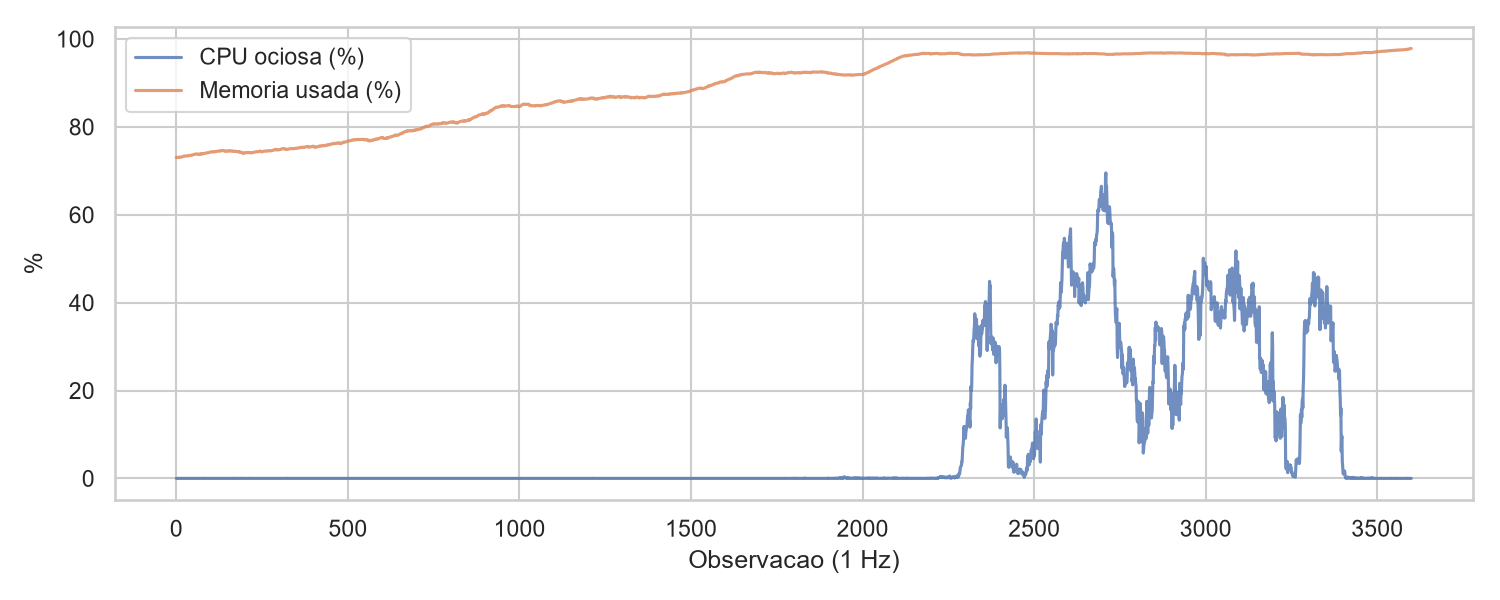
\includegraphics[width=\textwidth]{figs/task_i_3a_timeseries_cpu_mem.png}
    \caption{Série temporal de CPU ociosa e memória usada.}
    \label{fig:ts_cpu_mem}
  \end{subfigure}
  \hfill
  \begin{subfigure}[b]{0.48\textwidth}
    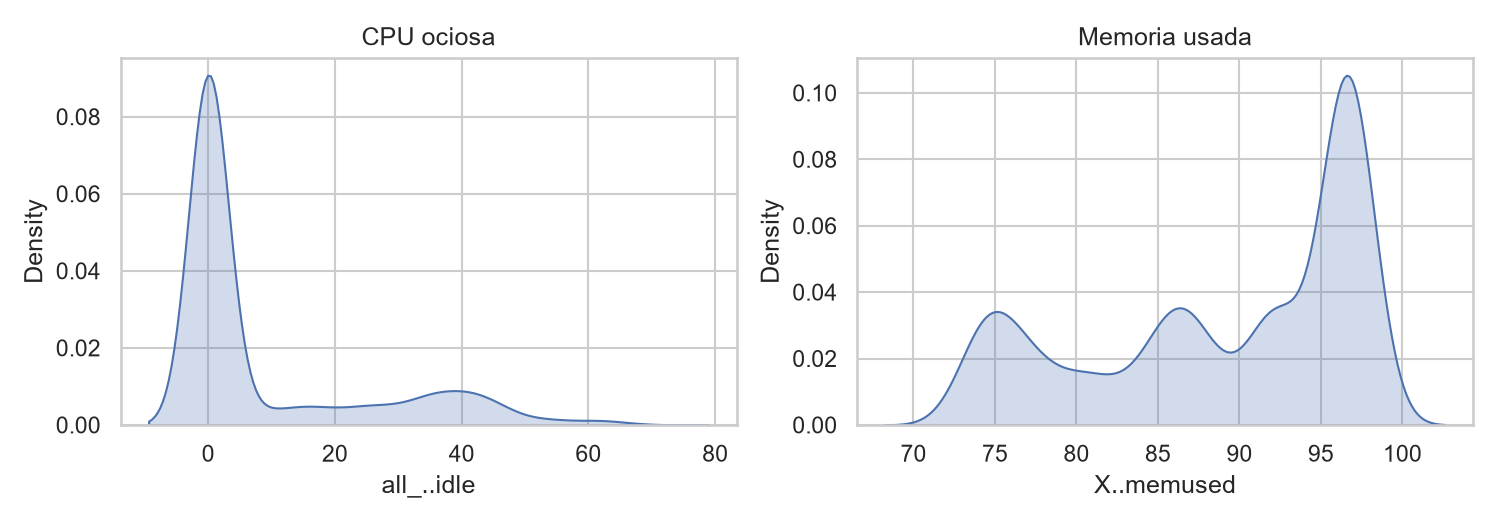
\includegraphics[width=\textwidth]{figs/task_i_3b_kde_cpu_mem.png}
    \caption{KDE de CPU ociosa e memória usada.}
    \label{fig:kde_cpu_mem}
  \end{subfigure}
  \caption{Comportamento das métricas do servidor ao longo do trace (Task~I).}
  \label{fig:task_i}
\end{figure}

A Figura~\ref{fig:ts_cpu_mem} mostra que a CPU ociosa apresenta grande variabilidade
ao longo do tempo, com picos e vales frequentes, enquanto a memória permanece estável
e elevada. O KDE (Figura~\ref{fig:kde_cpu_mem}) revela que a CPU ociosa possui distribuição
multimodal (com concentração entre 0--10\%), ao passo que a memória tem distribuição
estreita centrada em torno de 89\%, confirmando o comportamento observado nas estatísticas.

%% ============================================================
\section{Task II -- Regressão Linear}
%% ============================================================

\subsection{Objetivo e Métrica}

O objetivo é estimar \texttt{DispFrames} (valor contínuo) a partir das 9 variáveis do servidor.
A métrica de avaliação é o \textbf{NMAE} (Normalized Mean Absolute Error):

\begin{equation}
  \text{NMAE} = \frac{1}{\bar{y}} \cdot \frac{1}{m} \sum_{i=1}^{m} |y_i - \hat{y}_i|
\end{equation}

onde $\bar{y}$ é a média de \texttt{DispFrames} no conjunto de teste e $m = 1.080$.
O critério do enunciado é NMAE $< 15\%$.

\subsection{Implementação}

\begin{lstlisting}[caption={Treinamento e avaliação do modelo de regressão linear.}]
from sklearn.linear_model import LinearRegression
from src.metrics import nmae

model = LinearRegression()
model.fit(X_train, y_train)
y_pred = model.predict(X_test)

error = nmae(y_test, y_pred)   # NMAE normalizado pela media de y_test
\end{lstlisting}

\subsection{Coeficientes do Modelo M (treino completo)}

\begin{table}[H]
\centering
\caption{Coeficientes do modelo de regressão linear treinado com 2.520 observações.}
\label{tab:coef_reg}
\begin{tabular}{lr}
\toprule
\textbf{Variável} & \textbf{Coeficiente ($\Theta$)} \\
\midrule
CPU ociosa (\%)                  & $-0{,}0921$ \\
Memória usada (\%)               & $-0{,}0868$ \\
Média de carga --- 1 min         & $-0{,}0606$ \\
Sockets TCP em uso               & $-0{,}0653$ \\
Taxa de criação de processos     & $-0{,}0120$ \\
File handles em uso              & $-0{,}0031$ \\
Taxa de trocas de contexto       & $\approx 0$ \\
Taxa de interrupções             & $\approx 0$ \\
Taxa de liberação de páginas     & $\approx 0$ \\
\textbf{Intercepto ($\Theta_0$)} & $\mathbf{49{,}69}$ \\
\bottomrule
\end{tabular}
\end{table}

Todos os coeficientes significativos são negativos, indicando que maiores valores de
pressão no servidor (memória ocupada, carga de CPU, sockets ativos) estão associados
a estimativas menores de taxa de frames. O intercepto de 49,69 representa o valor
esperado de \texttt{DispFrames} quando todas as variáveis estão zeradas -- um valor
de referência sem interpretação física direta, dado que as variáveis não assumem valor
nulo na prática.

\subsection{Resultados por Tamanho de Treino}

\begin{table}[H]
\centering
\caption{NMAE e tempo de treino em função do tamanho do conjunto de treino.}
\label{tab:nmae}
\begin{tabular}{rrcc}
\toprule
\textbf{Obs. de treino} & \textbf{Tempo (ms)} & \textbf{NMAE (\%)} & \textbf{Acurado?} \\
\midrule
   50 & 1,1 & 11,52 & Sim \\
  500 & 1,9 & 10,58 & Sim \\
1.000 & 1,2 & 10,49 & Sim \\
1.500 & 1,2 & 10,38 & Sim \\
\textbf{2.520} & \textbf{2,6} & \textbf{10,39} & \textbf{Sim} \\
\bottomrule
\end{tabular}
\end{table}

\begin{figure}[H]
  \centering
  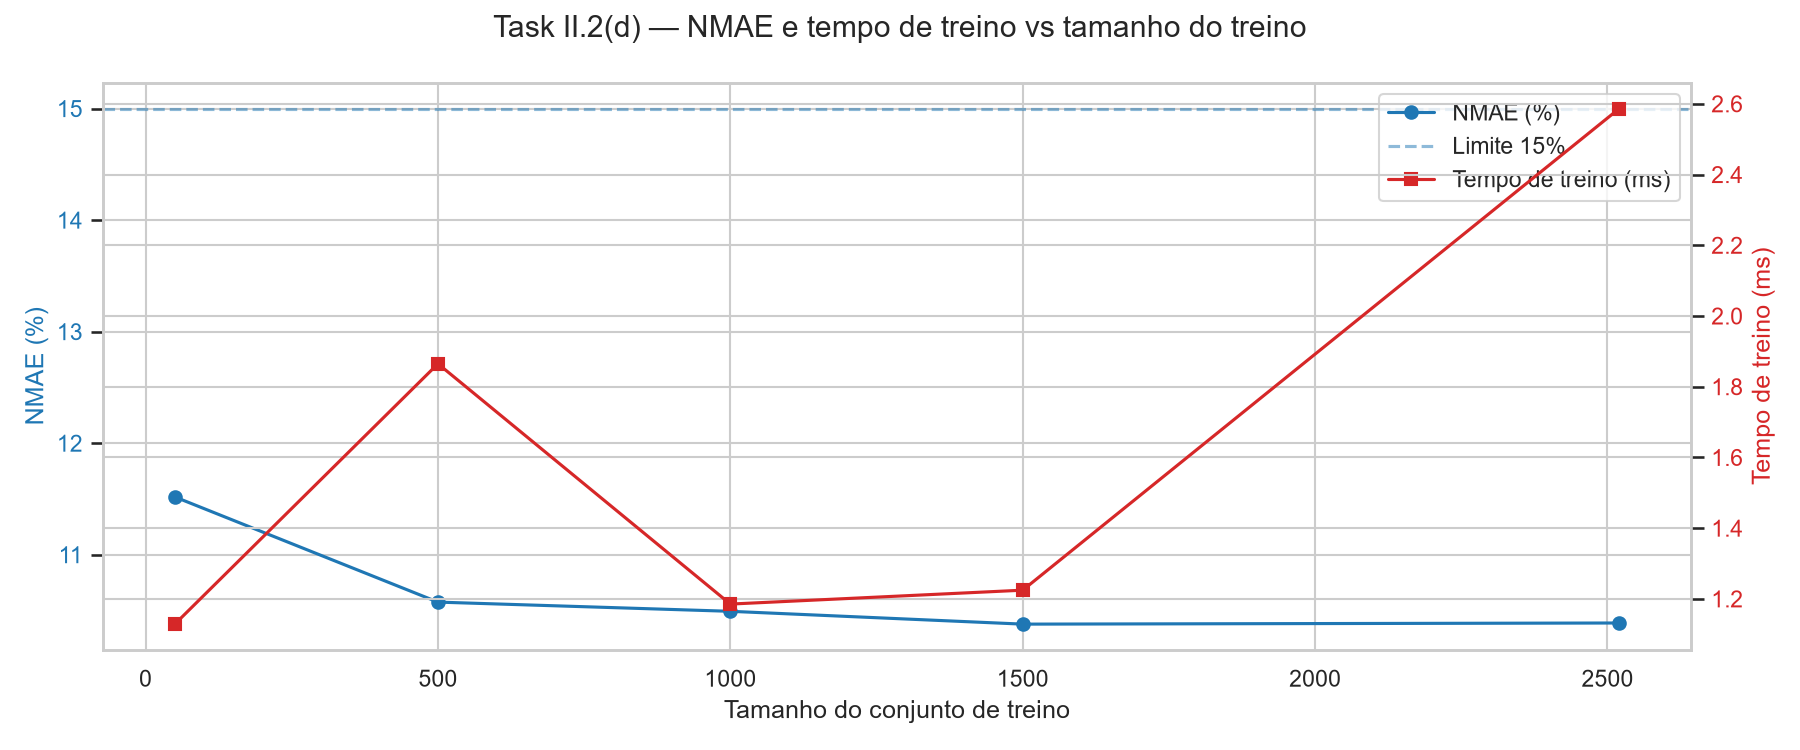
\includegraphics[width=0.6\textwidth]{figs/task_ii_2d_nmae_train_time.png}
  \caption{NMAE e tempo de treino em função do número de observações de treino (Task~II).}
  \label{fig:nmae_train}
\end{figure}

A Figura~\ref{fig:nmae_train} mostra que, mesmo com apenas 50 amostras, o modelo
já atinge NMAE $= 11{,}52\%$, abaixo do limiar de 15\%. O ganho de acurácia ao
aumentar o treino de 500 para 2.520 observações é inferior a 0,2 pp, caracterizando
\textbf{retornos decrescentes}. O tempo de treino permanece sub-milissegundo a poucos ms,
irrelevante para a decisão de tamanho.

\subsection{Análise no Conjunto de Teste}

\begin{figure}[H]
  \centering
  \begin{subfigure}[b]{0.48\textwidth}
    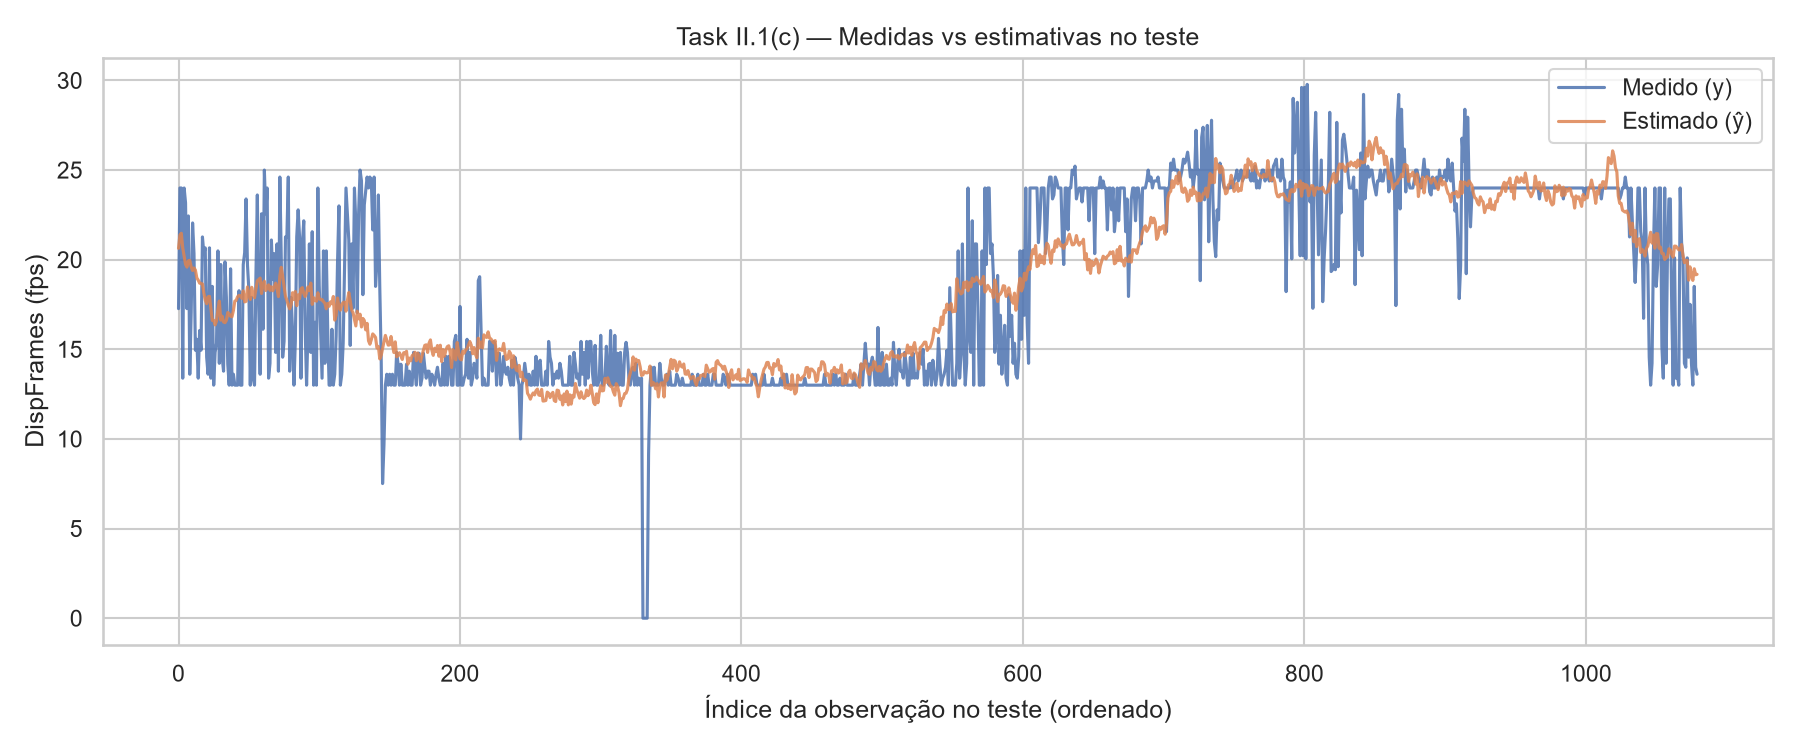
\includegraphics[width=\textwidth]{figs/task_ii_1c_timeseries_test.png}
    \caption{Série temporal: medido vs.\ estimado.}
  \end{subfigure}
  \hfill
  \begin{subfigure}[b]{0.48\textwidth}
    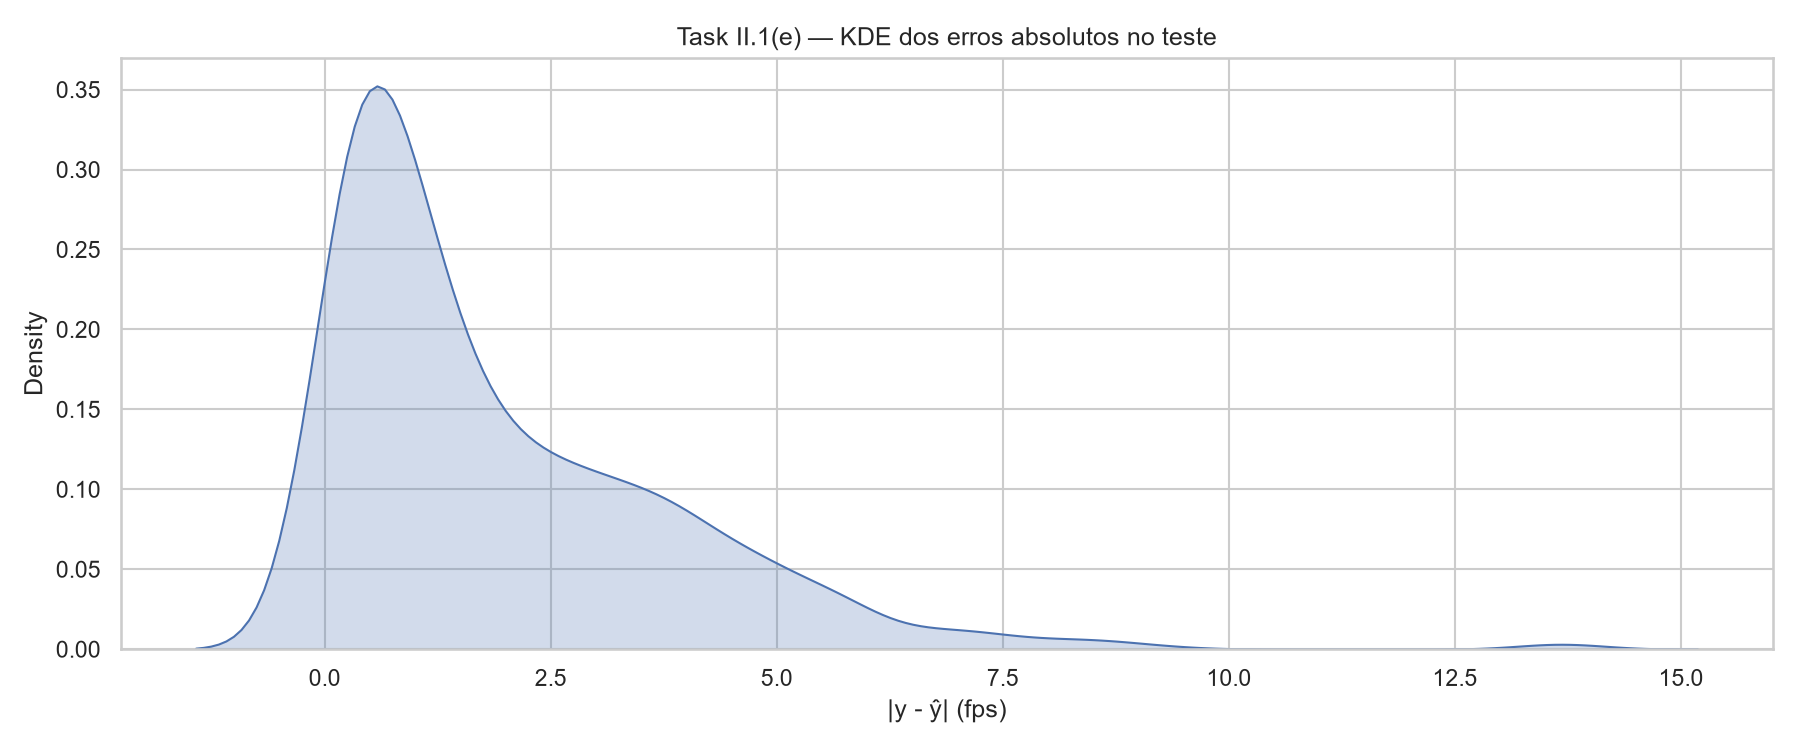
\includegraphics[width=\textwidth]{figs/task_ii_1e_kde_abs_errors.png}
    \caption{KDE dos erros absolutos $|y - \hat{y}|$.}
  \end{subfigure}
  \caption{Avaliação do modelo de regressão linear no conjunto de teste (Task~II).}
  \label{fig:reg_test}
\end{figure}

A série temporal (Figura~\ref{fig:reg_test}a) mostra que o modelo acompanha a tendência
geral dos fps, errando mais nos picos e vales -- onde a taxa de frames muda abruptamente.
O KDE dos erros absolutos (Figura~\ref{fig:reg_test}b) confirma que a maioria dos erros
se concentra abaixo de 5 fps, com cauda longa em eventos extremos.
O NMAE do modelo completo é \textbf{10,39\%}, abaixo do limite de 15\%.

%% ============================================================
\section{Task III -- Regressão Logística}
%% ============================================================

\subsection{Objetivo e Métrica}

Em vez de prever os fps exatos, o objetivo aqui é classificar cada instante como:
\begin{itemize}
  \item \textbf{Classe 1 (conforme):} \texttt{DispFrames} $\geq 18$ fps;
  \item \textbf{Classe 0 (violação):} \texttt{DispFrames} $< 18$ fps.
\end{itemize}

A métrica é o \textbf{ERR} (taxa de classificação errada):
\begin{equation}
  \text{ERR} = 1 - \frac{VP + VN}{m}
\end{equation}
onde VP = verdadeiros positivos, VN = verdadeiros negativos e $m = 1.080$.
O critério é ERR $< 15\%$.

\subsection{Implementação}

\begin{lstlisting}[caption={Criação dos rótulos e treinamento do classificador.}]
from sklearn.linear_model import LogisticRegression
from src.metrics import classification_error, sla_labels

# binariza Y: 1 se conforme, 0 se violacao
y_bin = sla_labels(y, SLA_THRESHOLD_FPS)

clf = LogisticRegression(max_iter=10000, random_state=RANDOM_STATE)
clf.fit(X_train, y_bin_train)
y_pred = clf.predict(X_test)

err = classification_error(y_bin_test, y_pred)
\end{lstlisting}

\subsection{Balanceamento das Classes}

No split de treino, aproximadamente 52\% das observações são conformes e 48\%
em violação. No conjunto de teste, a proporção é 50/50. O balanceamento razoável
entre as classes valida o uso de ERR como métrica primária.

\subsection{Resultados}

\begin{table}[H]
\centering
\caption{Resultados dos classificadores C1--C5 no conjunto de teste.}
\label{tab:class_results}
\begin{tabular}{rrrccrrrr}
\toprule
\textbf{Classif.} & \textbf{Treino} & \textbf{Tempo (ms)} & \textbf{ERR (\%)} & \textbf{Acurado?} & \textbf{VP} & \textbf{VN} & \textbf{FP} & \textbf{FN} \\
\midrule
C1 &    50 &  119 & 15,37 & N\~{a}o & 438 & 476 & 59 & 107 \\
C2 &   500 &  275 & 12,96 & Sim & 465 & 475 & 60 &  80 \\
C3 & 1.000 &  262 & 12,87 & Sim & 464 & 477 & 58 &  81 \\
C4 & 1.500 & 1373 & 11,39 & Sim & 479 & 478 & 57 &  66 \\
\textbf{C5} & \textbf{2.520} & \textbf{2527} & \textbf{11,11} & \textbf{Sim} & \textbf{486} & \textbf{474} & \textbf{61} & \textbf{59} \\
\bottomrule
\end{tabular}
\end{table}

C1 (50 amostras) não atinge o critério de 15\%, ficando no limite. A partir de C2 (500 amostras),
todos os classificadores são acurados. C5 obtém o melhor ERR: \textbf{11,11\%}.
O FN (serviço classif.\ como conforme quando viola) cai de 107 (C1) para 59 (C5),
o que é importante do ponto de vista operacional -- falsos negativos levam o provedor
a não agir em situações de violação real.

\subsection{Visualizações}

\begin{figure}[H]
  \centering
  \begin{subfigure}[b]{0.48\textwidth}
    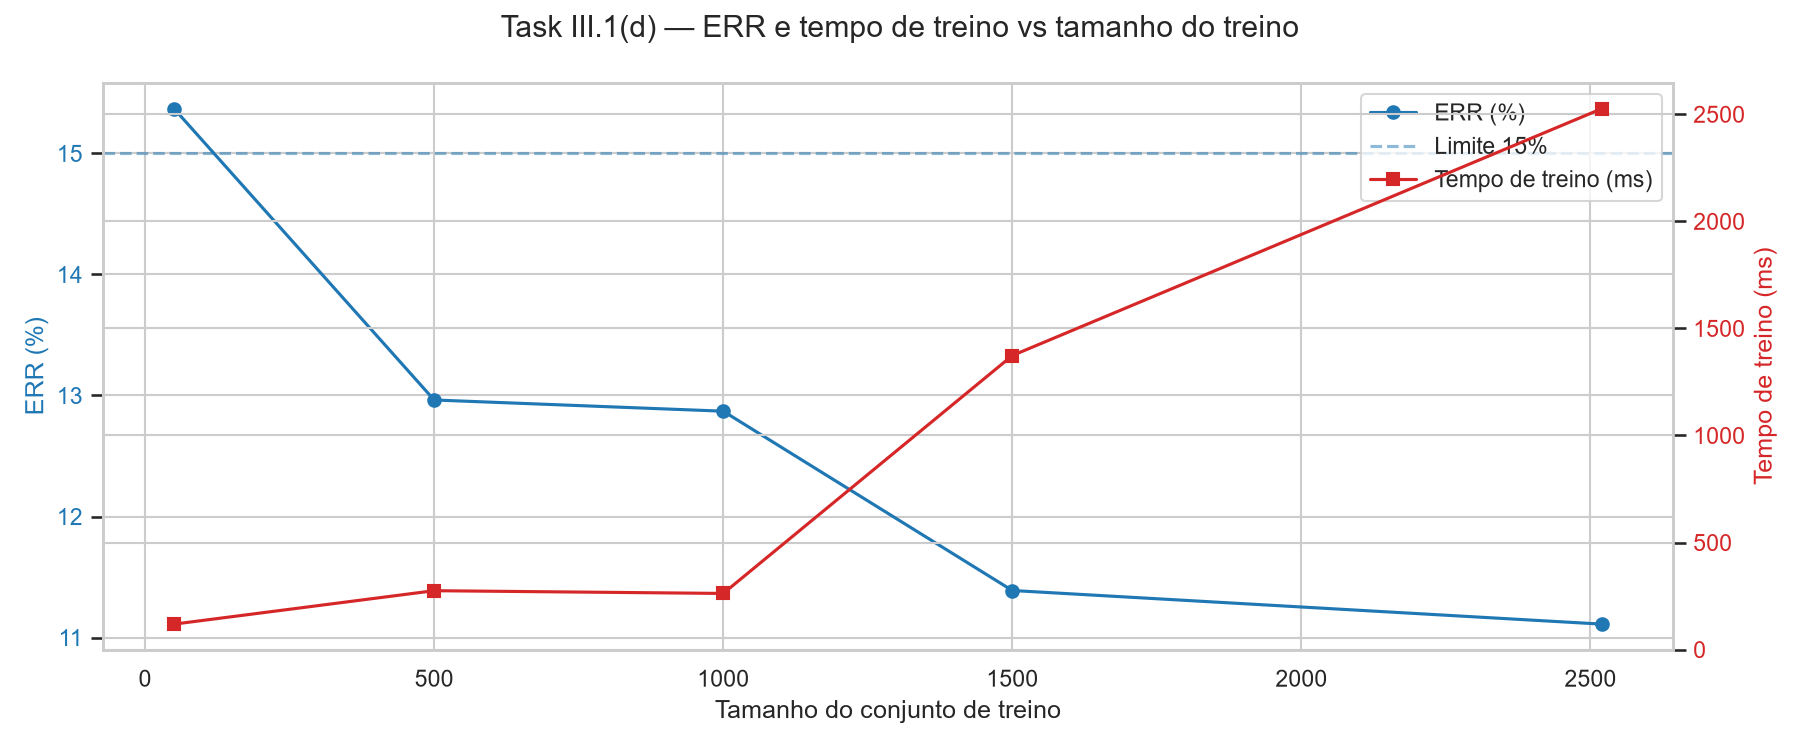
\includegraphics[width=\textwidth]{figs/task_iii_1d_err_train_time.png}
    \caption{ERR e tempo de treino vs.\ tamanho do treino.}
  \end{subfigure}
  \hfill
  \begin{subfigure}[b]{0.48\textwidth}
    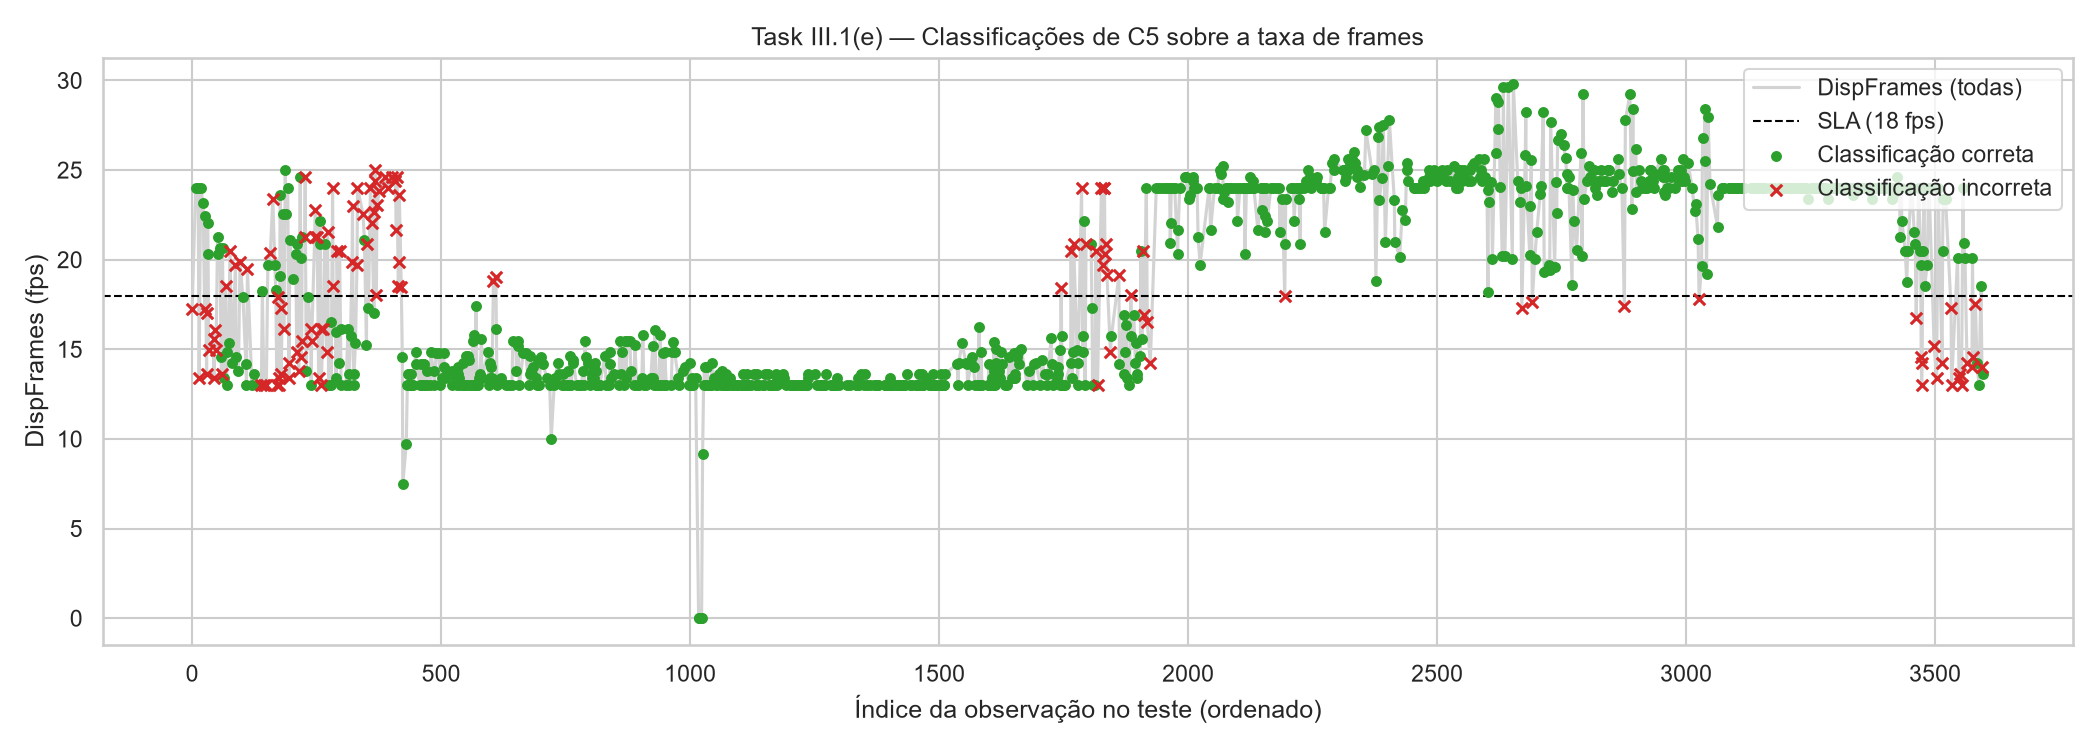
\includegraphics[width=\textwidth]{figs/task_iii_1e_timeseries_classification.png}
    \caption{Classificação de C5 no teste (verde = acerto, vermelho = erro).}
  \end{subfigure}
  \caption{Resultados da regressão logística (Task~III).}
  \label{fig:class_results}
\end{figure}

A Figura~\ref{fig:class_results}a confirma a tendência decrescente do ERR com mais dados,
com ganho expressivo entre 50 e 500 amostras e retornos decrescentes a partir daí.
O tempo de treino cresce mais acentuadamente de 1.500 para 2.520 amostras, refletindo
a natureza iterativa da regressão logística.

A Figura~\ref{fig:class_results}b mostra que os erros do melhor classificador (C5)
se concentram próximos ao limiar de 18 fps -- região onde a separação entre as classes
é intrinsecamente difícil. Longe do limiar, o modelo classifica corretamente com
alta consistência.

%% ============================================================
\section{Atividade Bônus -- 5G Datasets Challenge (Atividade A)}
%% ============================================================

\subsection{Descrição}

Como atividade opcional, foi implementada a \textbf{Atividade A} do 5G Datasets Challenge
(SMARTNESS/UNICAMP): predição de qualidade de sinal (\texttt{Qual}/RSRQ, em dB) a partir
de métricas de rede coletadas com Samsung S21 5G na rede Claro em São Paulo.

Foram utilizados três traces do dataset \texttt{g-nettrack-pro}:

\begin{table}[H]
\centering
\caption{Traces utilizados na Atividade Bônus.}
\label{tab:traces}
\begin{tabular}{ll}
\toprule
\textbf{Arquivo} & \textbf{Cenário} \\
\midrule
\texttt{2023-01-21\_308-walking-paulista-1.txt} & Pedestre -- Av.\ Paulista \\
\texttt{2023-01-22\_933-driving-sp-1.txt}       & Veículo em deslocamento \\
\texttt{2023-01-21\_244-subway-1.txt}           & Metrô \\
\bottomrule
\end{tabular}
\end{table}

As features utilizadas foram: \texttt{Level} (RSRP, dBm), \texttt{SNR},
\texttt{DL\_bitrate} (kbps), \texttt{UL\_bitrate} (kbps) e \texttt{Speed} (km/h).
Após remoção de valores inválidos (\texttt{--}, \texttt{-99}), restaram $\approx 4.500$
registros. O mesmo protocolo de split 70/30 com \texttt{random\_state=42} foi aplicado.

\subsection{Resultados}

\begin{table}[H]
\centering
\caption{Métricas do modelo de regressão linear para predição de \texttt{Qual} (5G).}
\label{tab:bonus_metrics}
\begin{tabular}{llp{7cm}}
\toprule
\textbf{Métrica} & \textbf{Valor} & \textbf{Interpretação} \\
\midrule
MAE  & 3,20 dB & Erro médio absoluto entre \texttt{Qual} medido e estimado \\
RMSE & 3,80 dB & Raiz do EQM -- penaliza erros grandes \\
R²   & 0,29    & Fração da variância de \texttt{Qual} explicada pelo modelo \\
\bottomrule
\end{tabular}
\end{table}

O coeficiente de determinação $R^2 = 0{,}29$ indica relação parcial -- esperado para
um modelo linear simples aplicado a dados heterogêneos que combinam cenários de
pedestre, veículo e metrô (indoor/outdoor), com eventos de handover não modelados.
A variável SNR é a de maior influência ($\Theta = +0{,}346$): maior relação
sinal-ruído está associada a melhor qualidade de sinal estimada.

\begin{figure}[H]
  \centering
  \begin{subfigure}[b]{0.48\textwidth}
    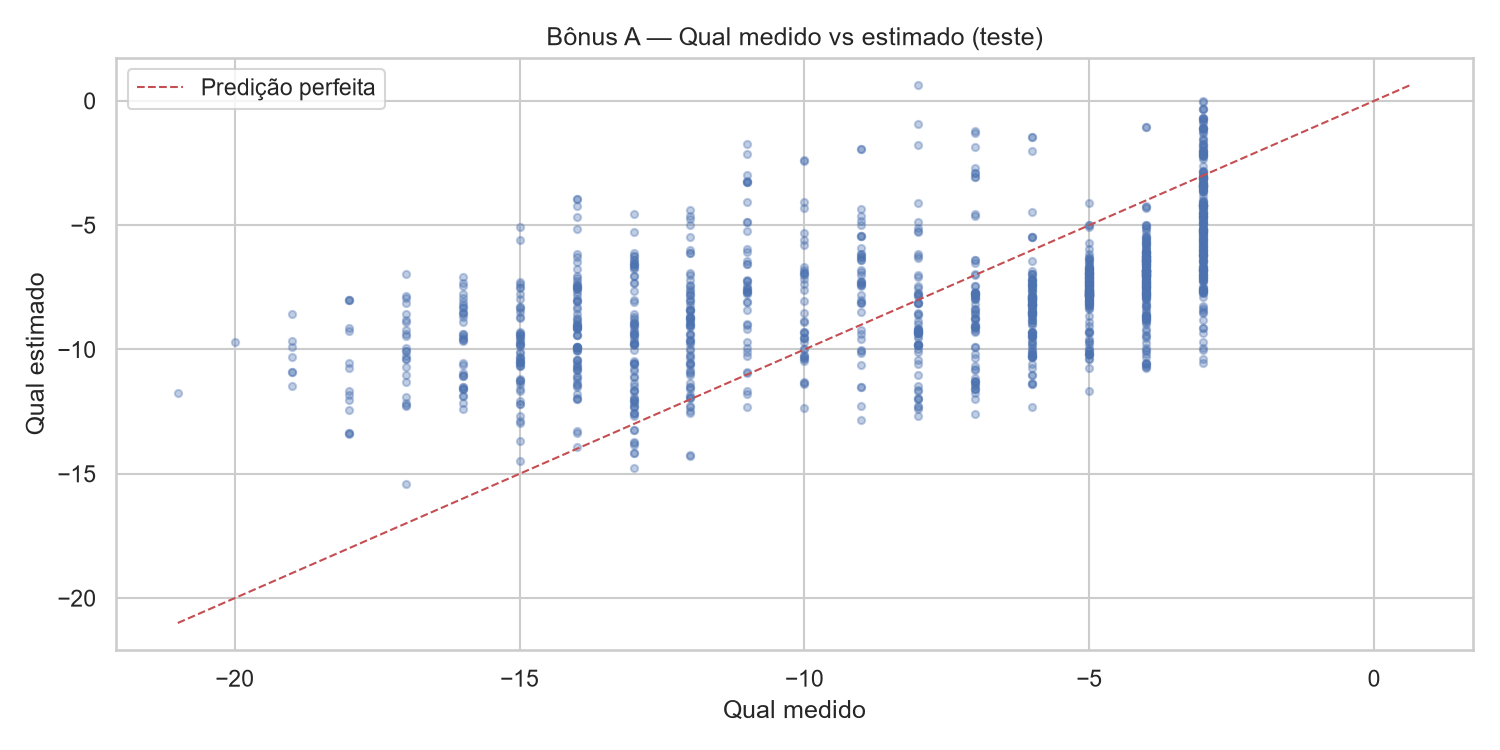
\includegraphics[width=\textwidth]{figs/bonus_a_qual_scatter.png}
    \caption{\texttt{Qual} medido vs.\ estimado.}
  \end{subfigure}
  \hfill
  \begin{subfigure}[b]{0.48\textwidth}
    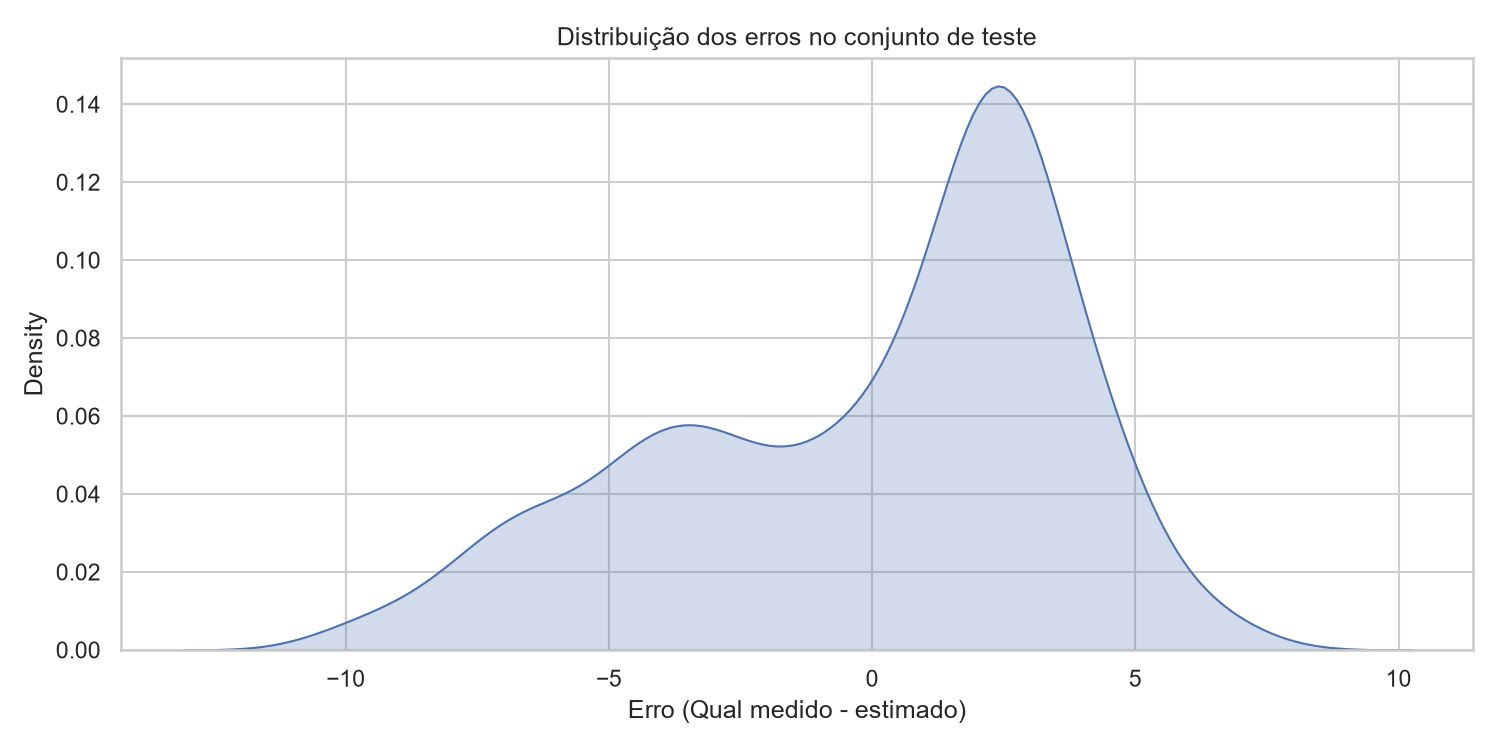
\includegraphics[width=\textwidth]{figs/bonus_a_erros_kde.png}
    \caption{KDE dos erros de estimativa.}
  \end{subfigure}
  \caption{Avaliação do modelo de predição de qualidade de sinal 5G (Atividade Bônus).}
  \label{fig:bonus}
\end{figure}

O scatter plot (Figura~\ref{fig:bonus}a) mostra dispersão considerável em torno da diagonal,
confirmando $R^2$ moderado. O KDE dos erros (Figura~\ref{fig:bonus}b) apresenta distribuição
aproximadamente simétrica centrada em zero, sem viés sistemático de superestimação ou
subestimação -- o modelo erra de forma equilibrada, o que é desejável.

%% ============================================================
\section{Conclusão}
%% ============================================================

Este trabalho demonstrou a viabilidade de usar modelos lineares supervisionados para
estimar conformidade a SLAs em serviços VoD a partir de métricas do servidor.

Na Task~II, a regressão linear atingiu NMAE de \textbf{10,39\%} (abaixo do limite de 15\%),
com retornos decrescentes a partir de 500 amostras de treino. Na Task~III, o melhor
classificador logístico (C5) obteve ERR de \textbf{11,11\%}, com os erros concentrados
na fronteira de 18 fps -- região inerentemente ambígua.

As principais limitações são: (i) a linearidade dos modelos, que pode não capturar
relações não lineares; (ii) o split aleatório, que pode misturar padrões temporais;
e (iii) a ausência de features de rede e do terminal do cliente.

Como trabalho futuro, propõe-se o uso de modelos não lineares (Random Forest, XGBoost),
validação temporal e enriquecimento das features com métricas de rede.

Na atividade bônus, a mesma metodologia aplicada a traces 5G obteve $R^2 = 0{,}29$,
resultado modesto mas interpretável para um baseline linear com dados de campo heterogêneos.

O código-fonte completo, notebooks reproduzíveis e dados estão disponíveis em:\\
\url{https://github.com/victorguimaraessilva/Trabalho-IA-MSc}

\end{document}
